\section{Requirements}
\textit{To provide secure and yet inconspicuous communication:}
\begin{enumerate}
    \item The system should be able to send messages through some social media.
    \item Messages, sent by the system, should not clearly seem to be a message, in the first place.
    \item The product should not require any personal information itself.
    \item The product should not take longer than 1 minute to install.
    \item 8 out of 10 users should clearly know (after installation) how the product preserves their privacy.
    \item The system should be able to receive and display messages sent by other users.
    \item 9 out of 10 users have to feel that their messages have been securely delivered.
    \item Users have to be able to chain messages together.
\end{enumerate}
\noindent
The first requirement is based on the fact that every persona uses an average of 7-8 different social media a day, thereby a good use for the product could be on any or multiple social media.\\
The second requirement for the product has to be met, as the product otherwise would not enhance the privacy of the individual user.\\
The concerned user [Persona 2] would be highly unwilling to provide any personal information and this leads to the third requirement as they otherwise might not be willing to use the product.\\
\newpage\noindent
The forth requirement regards The user [persona 3] as these would only use the product if it would not require a greater effort.\\
The fifth requirement helps to attract both The concerned and the non concerned [Persona 1 \& 2] as these are both interested in the enhancement of their security but especially the concerned would only use the product if he could see and understand the actual benefit.\\
The sixth requirement is a basic requirement as the product otherwise wouldn't have any use.\\
The seventh requirement is important as the product needs to provide the different users, especially the concerned [Persona 2], with this feeling, as the user otherwise, with particular focus on the normal user [Persona 3], wouldn't use the product more than once.\\
Lastly users like [Persona 2] require the product to function like any other social media, in that they are able to comment and write to each other based on the different posts in relation to one and each other.

\section{Prototype}

\begin{table}[H]
    \begin{minipage}{.5\textwidth}
        \begin{figure}[H]
            \centering
            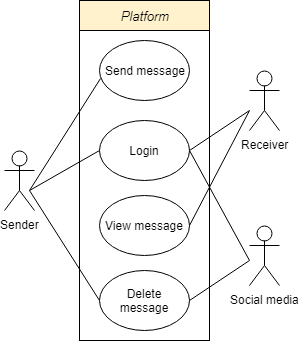
\includegraphics[width=0.75\linewidth]{Projectdoc/Assets/Illustrationer/simple-usecase-eng.png}
            \caption{Usecase diagram}
            \label{fig:usecase}
        \end{figure}
    \end{minipage}
    \begin{minipage}{.5\textwidth}
        \noindent
        Figure \ref{fig:usecase} on the left  describes a conceptual model of what the basic functionality of the inconspicuous communication platform looks like. The model describes how a sender, receiver and a external social media will interface with the system. The "Send message" action will be interfaced with by the sender and will deliver the message to the system for further processing. The "Login" action connects the sender, receiver and social media together. The "View message" action will be interfaced with by the receiver and displays a message from the system. The "Delete message" will be interfaced with by both the sender and the social media and will trigger a message deletion request to the system.
    \end{minipage}
\end{table}

\textbf{Use case \#1, Login.}\\
Object: The user should be prompted for a login, either through a personal social media, or though an anonymous bot.\\
Attributes: Selection of bot, Social media credentials.\\
Operations: Connect the user through the given credentials.\\
Manipulation: Set default settings through sub tap,  Set remember login credentials with checkbox.\\
Next Relationship: Send message[\#2], View message[\#3].\\\\
\newpage
\noindent
\textbf{Use case \#2, Send message.}\\
Object: The user has the option to select a category or thread to submit a new message.\\
Attributes: Selection of post relations, message content.\\
Operations: Post user generated message in relation to the selected thread or category.\\
Manipulation: None.\\
Next Relationship: Login[\#1], Send message[\#2], View message[\#3].\\\\
\noindent
\textbf{Use case \#3, View message.}\\
Object: The user has the option to select a specific message or thread to display.\\
Attributes: Category, Message, Thread.\\
Manipulation: Option to delete a message or thread (If user has ownership).\\
Next Relationship: Login[\#1], Send message[\#2], View message[\#3], Delete message[\#4].\\\\
\noindent
\textbf{Use case \#4, Delete message.}\\
Object: The user have the option to select a specefic message or thread to delete (if user contains ownership).\\
Attributes: Message, Thread, Ownership.\\
Manipulation: Delete a message or thread.\\
Next Relationship: Login[\#1], Send message[\#2], View message[\#3].\\